\section{Problèmes rencontrés, problèmes résolus}

Le développement de GuitarTutor ne s'est pas fait sans heurts. Nous sommes néanmoins parvenus à résoudre les différents problèmes auxquels nous avons été confrontés au cours des phases de développement.

\subsection{Reprise de code}

Comme c'était prévu, la reprise du code existant fut notre première grande étape de développement. Passé le moment de découragement lié à l'absence total de commentaires et de documentation dans la grande majorité du code source qui nous intéressait, nous nous sommes attelés à ``débroussailler'' le dépôt en mettant en place une documentation, en commentant le code, ainsi qu'en supprimant purement et simplement les portions inutilisées, qui représentaient tout de même une quantité de code loin d'être négligeable (parfois de simples fonctions, parfois des fichiers, et parfois des dossiers entiers\dots).

Par ailleurs, du fait que le projet ait été constitué de plusieurs blocs de code émanant de différentes équipes de développeurs, nous avons pu remarquer que les conventions de codage n'avaient pas été harmonisées. Nous avons pris soin de réparer cette erreur afin de faciliter la relecture et donc la réutilisation de ce même code. Les outils de refactorisation de Qt, bien qu'imparfaits, nous ont été particulièrement
utiles, en permettant par exemple la transformation d'un nom de variable en camelCase, répercuté sur toutes ses utilisations.

Passés ces quelques semaines de nettoyage et d'assimilation du code existant, nous avons pu commencer à apporter les modifications établies dans le cahier des charges, bien que, tout au long du développement, nous ayons continué la refactorisation (par exemple les suppressions de certaines bibliothèques, évoquées plus loin dans ce rapport).

\subsection{Refonte de l'interface du lecteur}

La refonte totale de l'interface du lecteur s'est présentée comme un véritable défi. Il s'agissait en effet de supprimer tout ce qui concernait l'interface dans le projet existant, et d'y mettre à la place notre propre code. Évidemment, il n'était pas question de se limiter à une structure identique à l'interface existante, celle-ci étant véritablement limitée en terme de fonctionnalités, voire clairement repoussante pour un jeune guitariste débutant. Fort heureusement, le lecteur était déjà plut\^ot bien décomposé selon le modèle \ac{MVC}, ce qui nous a tout de m\^eme motivés à tenter l'expérience.

La nouvelle interface a donc initialement été développée seule, totalement séparée du reste du projet, en utilisant des faussaires pour simuler une grille d'accords, et ce, selon une maquette que nous avions soumise à nos clients (voir figure \ref{annexe_proto_player} en annexe). Ce n'est qu'au bout de plusieurs semaines de développement que nous avons enfin pu intégrer la nouvelle interface au reste du projet. Cette intégration ne s'est pas faite sans heurts, mais a finalement aboutie, comme nous l'espérions (voir figure \ref{interface_player}).

\begin{figure}[H]
\begin{center}
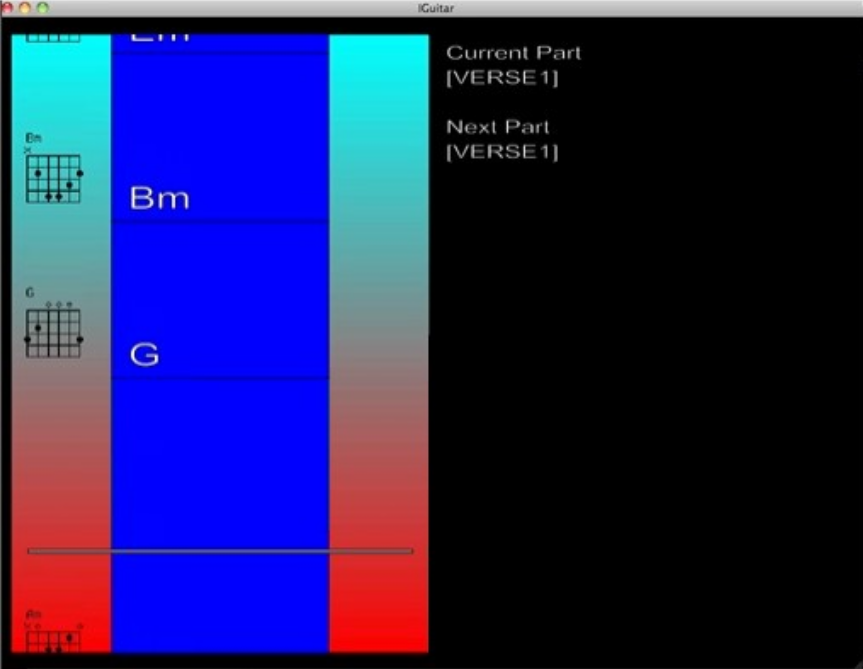
\includegraphics[width=175px]{ancien_player.png}
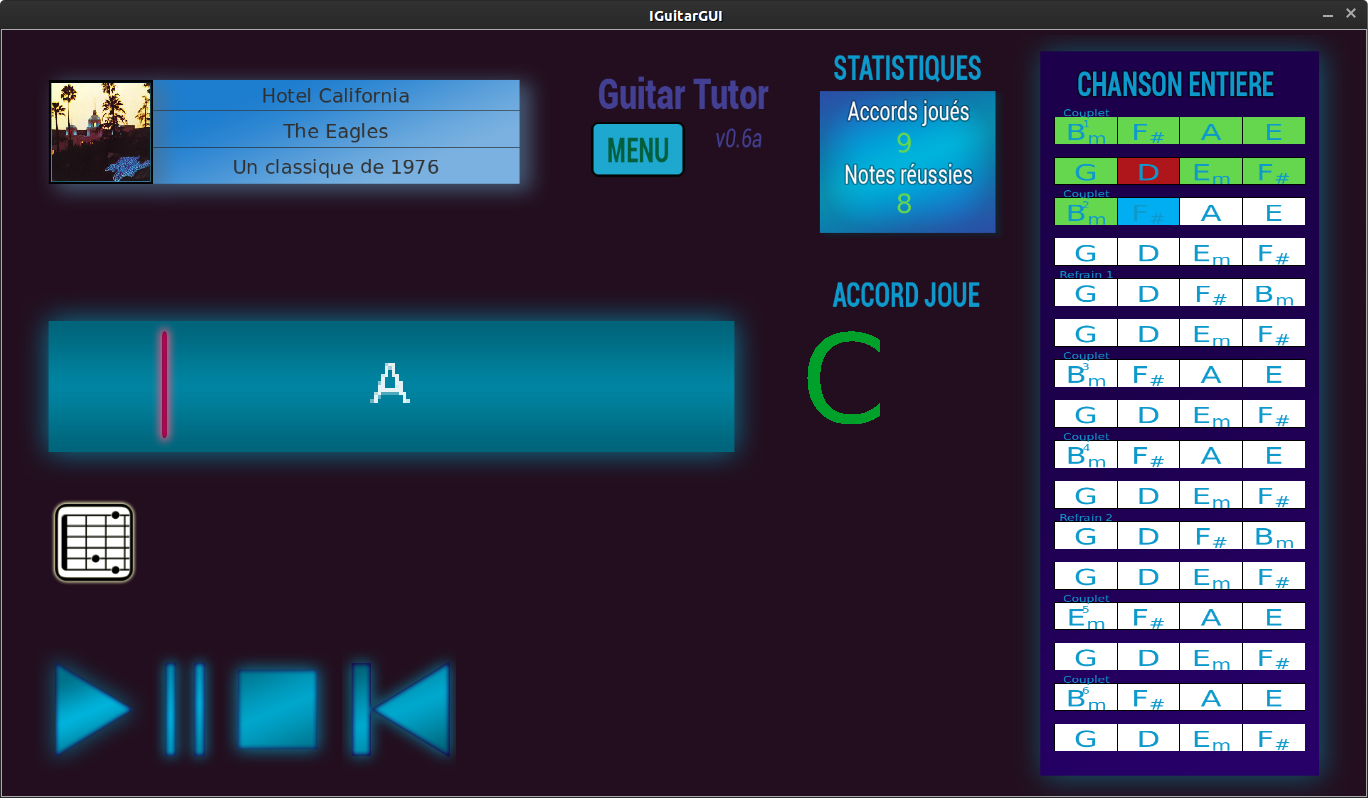
\includegraphics[width=275px]{interface_player.png}
\caption{L'interface du lecteur a été entièrement refaite}
\label{interface_player}
\end{center}
\end{figure}

\subsection{Portabilité}

La portabilité du logiciel, notamment sur Mac OS et Windows, faisait partie des principales demandes des clients. Les librairies utilisées jusque là était censées fonctionner à la fois sur Mac OS, Windows et GNU/Linux, et c'était une bonne raison pour ne pas en changer.

Nous nous sommes cependant rapidement rendus à l'évidence: on ne développe pas un logiciel portable simplement en utilisant des librairies portables.

\subsubsection*{Sur Mac OS}

Personne, dans notre équipe, n'ayant une machine sous Mac OS, nous avons dû nous contenter d'une version de Mountain Lion en machine virtuelle. Outre un problème d'extrême lenteur lors de la compilation et divers autres soucis liés à la connexion internet et la reconnaissance des ports USB, il était impossible de vérifier le bon fonctionnement du lecteur, puisque l'entrée audio de la VM n'était pas activée. Nous avons donc pendant longtemps développé \textit{``à l'aveugle''} sous Mac OS, où tout ce que nous pouvions faire était de vérifier que la compilation se faisait correctement.
Un temps d'adaptation a d'ailleurs été nécessaire car bien que la base du système repose sur Unix, l'ergonomie du système est très différente
de ce dont nous avons l'habitude.

Fort heureusement, un test sur une vraie machine Mac début mars nous a confirmé que le projet était bien compatible, et nous en avons également profité pour vérifier le fonctionnement de notre installateur.

Nous avons néanmoins connu des sueurs froides lors de l'intégration de la bibliothèque FMOD qui a pendant un temps causé des
problèmes sur les machines Mac réelles, alors que tout fonctionnait sous nos machines virtuelles. Cela a été l'occasion de découvrir
le système de paquetage utilisé sous Mac, ainsi que les outils qui permettent de s'en servir, comme \texttt{macdeployqt} et \texttt{install\_name\_tool}.

Enfin, s'est posé le problème du choix du compilateur. Il y a deux compilateurs principaux sous Mac : \ac{GCC} et Clang.
Néanmoins, le premier n'est plus réellement supporté par Apple : la version fournie par les outils de développement Apple est la 4.2,
alors que nous en sommes à la 4.7. Clang, en contrepartie, est issu du projet LLVM et est fortement soutenu par Apple.
Bien qu'il n'offre à ce jour pas toutes les fonctionnalités de \ac{GCC} (comme le support d'OpenMP, par exempl), il permet une
compilation très rapide et des performances parfois plus élevées que la dernière version de \ac{GCC} (et sensiblement plus élevées que la 4.2).
Nous avons donc décidé de retenir ce dernier pour les livrables.
\subsubsection*{Sur Windows}

Le portage sous Windows a été périlleux, car le système de base n'a rien à voir avec les systèmes ayant pour base Unix et respectant
les normes POSIX que sont Linux et Mac OS X.

Notre premier réflexe a été d'utiliser MinGW qui est livré par défaut avec Qt. Néanmoins, un problème
dans la librairie winpthreads qui était livré avec la version de MinGW qui était elle-même livrée avec Qt 4.8 nous a
forcé à passer sur la librairie BOOST C++ pour un temps. De plus, en raison de l'utilisation de certaines fonctionnalitées modernes
de \ac{GCC} 4.7 sous Linux, qui n'étaient pas disponibles sous MinGW 4.2, la compilation ne marchait pas sous Windows.

Nous effectuions donc un cross-compiling depuis Linux, ce qui représentait une certaine perte de temps pour les tests,
qui pour la plupart s'effectuaient d'ailleurs sous Wine, l'environnement de simulation Windows sous Linux.

Il a de plus fallu recompiler libsndfile qui n'était pas disponible directement sous Windows.

\paragraph{Arrivée de Qt5}
De ce point de vue, l'arrivée de Qt 5 a été salvatrice pour notre projet : en effet, elle mettait à jour MinGW
avec la dernière version de \ac{GCC}, la 4.7, ce qui a permis une compilation directe depuis Windows, ainsi que la suppression des
threads BOOST pour un retour aux pthreads.

Nous avons de plus travaillé sur une branche qui permette la compilation avec \ac{MSVC}, le compilateur C++ Microsoft.

Néanmoins, ce compilateur ne supporte pas le standard C99, qui est utilisé dans la librairie EHPCP pour représenter les types complexes.

Nous avons donc fait une tentative de portage en utilisant la classe C++ Complex, mais les performances étaient moindres au final,
ce qui nous a poussé à rester sous MinGW pour le rendu. Néanmoins, cela a été l'occasion d'apprendre les
bases de l'\ac{API} Windows, notamment pour la gestion des threads.

\paragraph{Installation}
Une des autres particularités de Windows est qu'il n'y a pas de système de gestion de paquetage comme sous la majorité des systèmes Linux et Mac OS X.
Il est donc nécessaire de créer nous-même un installeur, nous avons pour ce faire utilisé Advance Installer dans sa version gratuite.

Ce logiciel permet un déploiement facile : création d'icônes dans le menu démarrer, sur le bureau, gestion des mises à jour...

\paragraph{Portaudio et performance audio basse-latence}
Contrairement à Linux et Mac OS X, dont les couches audio ALSA (pour Linux) et CoreAudio (pour Mac OS X) permettent immédiatement
des basses latences, ce n'est pas le cas sous Windows.

Cela pose problème pour le jeu de guitare : en effet, la latence de base du mixeur Windows est d'environ 40 millisecondes.
Et des mesures ont montré que l'oreille humaine arrivait à percevoir un décalage à partir de 10 millisecondes, et que cela devenait gênant pour le jeu à partir de 20 millisecondes.

Une solution a été développée par Steinberg (l'éditeur du séquenceur Cubase) : le protocole ASIO.

Ce protocole permet d'atteindre de très basses latences (parfois jusqu'à moins d'une milliseconde) avec
du matériel professionnel et de basses latences avec ASIO4ALL, un logiciel qui permet d'utiliser des cartes son standard de PC avec le protocole ASIO.

Le problème pour l'incorporation de cette technologie dans le projet est qu'il est nécessaire de compiler PortAudio avec le SDK ASIO, ce qui
ne peut se faire qu'avec \ac{MSVC}, le compilateur Microsoft.
Comme l'algorithme de name-mangling de \ac{MSVC} est incompatible avec celui de MinGW / \ac{GCC}, il est nécessaire de recompiler tout le projet avec \ac{MSVC}, ce qui cause la perte de performance vue plus haut.
De plus, il faut remplacer la DLL portaudio fournie dans le livrable avec la DLL compilée avec le support ASIO, ce qui fait
que le logiciel ne pourra pas s'exécuter sur un ordinateur sans ASIO4ALL ou une carte son professionnelle fournissant un pilote ASIO.

\subsubsection*{Sur GNU/Linux}

Il s'agit du seul des trois systèmes d'exploitation pour lequel nous n'avons pas eu de problème particulier, mais aussi le seul qui n'était pas demandé. Peut-être est-ce simplement parce que nous avons tous commencé à coder directement sur celui-ci, et que c'est aussi le système sur lequel le groupe de PFA précédent s'était focalisé.

\subsubsection*{De l'avantage de l'utilisation de multiples compilateurs}

Bien qu'à priori, on puisse penser que c'est un calvaire de maintenir un même programme fonctionnel sur plusieurs systèmes et plusieurs compilateurs, nous nous sommes rendu comptes que cela avait aussi un avantage majeur : la détection d'erreurs et d'incorrections.
Ainsi, \ac{GCC} est parfois assez laxiste quand à son interprétation des standards du C++ et permet des choses qui ne sont pas toujours acceptées par les autres compilateurs.

L'utilisation de Clang et de \ac{MSVC} a donc permis de soulever des approximations qui étaient passées inaperçues sous \ac{GCC} mais qui contribuaient à avoir un code moins lisible.
De plus, cela nous a permis de comprendre de quelle manière l'interprétation des standards pouvait différer d'un compilateur à l'autre.

Enfin, nous avons pu mesurer des différences de performance : par exemple, sous Windows, aussi étrange que cela puisse paraître, l'exécution du lecteur nous a semblé beaucoup plus fluide lorsque compilé avec MinGW plutôt qu'avec \ac{MSVC} qui est pourtant le compilateur Microsoft. Toutes les optimisations possibles étaient activées dans les deux cas.

\subsection{Problèmes directement liés au code}
Nous parlerons ici de quelques problèmes directement liés à la programmation que nous avons rencontré tout au long du projet.

\subsubsection{L'apprentissage du C++}
Un des désavantages de notre emploi du temps est que nous commençons les cours de C++ \textit{après} le début du projet.

Ce n'est pas un problème pour ceux de l'équipe qui en ont déjà fait de leur côté mais c'est un désavantage certain pour les autres,
qui nuit grandement à la dynamique de groupe.

Ce serait sans doute moins visible dans un projet PFA standard ou les premiers mois sont entièrement dédiés à la conception
d'un cahier des charges, mais nous avons du nous plonger dans le code existant dès le début pour comprendre ce qu'il faudrait faire, et cela a parfois pu sembler difficile sans avoir les connaissances théoriques nécessaires à la compréhension de ce code.

\subsubsection{L'utilisation des cast}
Nous avons été confronté à un problème sur l'utilisation des cast:
Supposons que l'on ait un objet A, héritant de \texttt{QWidget} et possédant les propriétés de la macro \texttt{Q\_OBJECT}.
Cet objet A possède un lien a-un avec un objet B (A contient B).
B hérite aussi de \texttt{QWidget} et possède les propriétés de \texttt{Q\_OBJECT} comme cela :
\begin{figure}[H]
\begin{lstlisting}
class A : public QWidget
{
	Q_OBJECT
	public:
		A():  m_x(0)
		{
			m_B = new B(this);
		}

		int someAMethod()
		{
			return m_x;
		}

	private:
		B* m_B;
		int m_x;
}

class B : public QWidget
{
	public:
		B(QWidget* parent): QWidget(parent)
		{
			m_parent = parent;
		}

		someBMethod()
		{
			int z = ((A*) m_parent)->someAMethod(); // fonctionne très bien
			int z = ((A*) parent())->someAMethod(); // provoque l'apocalypse
		}

	private:
		QWidget* m_parent;
}
\end{lstlisting}
\caption{Calcul d'exponentielle complexe, extrait de \texttt{fft.c : butterfly}}
\label{api_cexp_computation}
\end{figure}

On pourrait penser que \texttt{B::z} vaudrait $0$, la valeur de \texttt{x}, à la fin d'un appel de \texttt{B::someBMethod}.
En réalité, le programme \textit{explose}. La mémoire devient corrompue, les objets
changent de type de manière aléatoire et les erreurs de segmentation se mettent à pleuvoir.

Le problème, comme il nous l'a été expliqué sur les forums Qt, repose en fait sur le cast de \texttt{parent()}
en A* (alors que cette méthode est sensée renvoyer le \texttt{QWidget*} parent avec lequel est fait l'initialisation).

Au lieu d'utiliser un cast standard, il est nécessaire d'utiliser les méthodes de cast propres au C++ :
\texttt{static\_cast}, \texttt{dynamic\_cast}, ou encore \texttt{qobject\_cast}, propre à Qt.

\subsubsection{L'apprentissage de Qt}
Qt est quasiment un langage à proprement parler, et il apport au C++ des fonctionnalités auxquelles nous n'étions pas habitués,
comme par exemple le mécanisme de signaux et slots.

Ainsi, vu que nous avons appris à nous en servir en cours de route, nous n'avons peut-être pas utilisé ce système au maximum de ses
capacités. Notamment, beaucoup de méthodes dans l'éditeur auraient pu être rendues superflues par une utilisation appropriée des signaux.
Un exemple de l'avantage des signaux est la mise à jour dynamique de l'interface, ce qui est très à la mode notamment avec
les interfaces mobiles. Par exemple, on peut voir qu'il n'y a pas de bouton "Appliquer" dans le panneau de configuration de l'éditeur :
les changements sont répercutés en temps réel sur le reste du programme.

Le principe de la délégation, notamment pour le dessin des \texttt{CaseItem} à l'aide de \texttt{CaseItemDelegate} a aussi mis un certain temps avant d'être entièrement compris.
Le lecteur étant plus récent dans sa conception, l'étude de son code permet de voir une meilleure compréhension des mécanismes de Qt,
bien que nos connaissances en la matière soient encore perfectibles.

\subsubsection{Le fonctionnement du système de ressources}
Il nous a fallu un certain temps pour comprendre comment fonctionnaient les ressources avec Qt :
le plus difficile a été d'arriver à inclure les fichiers d'aide directement dans le programme.

De plus, ce système de ressources n'est pas omnipotent : par exemple, pour avoir des icônes, il est
nécessaire de créer un fichier de ressource par système d'exploitation (voire par environnement : par exemple,
sous Linux, l'implémentation va différer entre Gnome, KDE, XFCE...).
